\subsection{Network Optimization}

The performance of any networked file system is fundamentally limited by the underlying network on which the file system communicates. The network's characteristics, such as latency and throughput, impose a theoretical upper bound on the file system's capabilities. To distinguish between the limitations imposed by Ceph's architecture and that of the network hardware, this section establishes our methodology for tuning network performance and establishing a throughput baseline.

Ceph deployments do not utilize \ac{RDMA} by default for communication, in contrast to \acs{HPC}-native file systems such as Lustre and BeeGFS. While \ac{RDMA} is a common feature in \ac{HPC} networking hardware, Ceph relies on the standard \ac{TCP/IP} stack for its communication. The use of \ac{TCP/IP} over \ac{RDMA} introduces several performance trade-offs~\cite{linux_kernel_networking}:

\begin{itemize}
    \item \ac{TCP/IP} processing is primarily performed in software, incurring significant performance costs at high throughputs through packet processing and context switching overhead.
    \item \ac{RDMA} performs zero-copy transfers, which allow for direct placement of data from the network adapter to application memory. However, \ac{TCP/IP} performs multiple buffer copies throughout the networking stack before reaching user space, incurring additional overhead.
    \item The aforementioned kernel overhead and memory copies lead to increased \ac{CPU} usage, reducing the compute performance available for \ac{HPC} workloads.
\end{itemize}

Consequently, Ceph incurs a \ac{CPU} utilization and network throughput disadvantage compared to \ac{HPC} file system competitors, inherent to its use of \ac{TCP/IP} for communication. Additionally, the modeling of \ac{TCP} performance can be more complex, as it depends on several additional factors beyond theoretical link speed:

\begin{itemize}
    \item Network type (Ethernet, InfiniBand, etc.)
    \item Kernel version and driver version, since newer kernels may have more optimized networking code
    \item Performance of the \ac{CPU}, including factors such as its clock speed, core count, memory layout, and internal interconnect bandwidth
    \item The offloads available and used on the network adapter
    \item Tunable parameters, such as:
    \begin{itemize}
        \item \ac{MTU}
        \item Congestion control algorithms
        \item Interrupt handling and steering
        \item Message buffer sizes
    \end{itemize}
\end{itemize}

While these factors can also affect \ac{RDMA} transports, the offloading of data transport operations to network hardware mitigates much of the performance variability which can arise from host-side bottlenecks. Therefore, in the context of this thesis, the performance baselines established are intended for comparative measurements on identical hardware, rather than an absolute metric for peak performance. The following subsections cover the optimizations applied to Omni-Path and InfiniBand, as these interconnects are used in the \ac{GWDG} \ac{HPC} cluster nodes.

\subsection{Omni-Path Optimizations}
\label{sec:opa-optimization}

The majority of the production nodes used in the \ac{HPC} cluster of the \ac{GWDG} are
equipped with Omni-Path networking, and a small number with InfiniBand
networking. However, we will focus primarily on Omni-Path, as it exhibited
architectural limitations which had a significant negative impact on the
\ac{TCP} performance available over the transport. We will focus on
the configuration and issues which were particularly impactful.

Initial testing was performed on the default Omni-Path configuration on the
\ac{GWDG} computing center. The results from these tests were poor, with 
inconsistent \ac{TCP} throughput of under 20 Gbps. The configuration and
performance results are unchanged from tests previously performed on the same
hardware~\cite{using-hpc-networks}. 

\subsubsection{Recommended Optimizations}

The Cornelis optimization guide for Omni-Path~\cite{omni-path-tuning-guide}
recommends tuning the following options in order to improve the performance of
\ac{TCP/IP} over the fabric:

\begin{itemize}
    \item Adjust the \ac{MTU} of the network interface\footnote{\cite[pp.~71--75]{omni-path-tuning-guide}}
    \item Enable \ac{GSO}\footnote{\cite[pp.~76--77]{omni-path-tuning-guide}}
    \item Enable either \ac{RPS}, or Accelerated \ac{IP} without \ac{RPS}\footnote{\cite[p.~77]{omni-path-tuning-guide}}
    \item Adjust the system \ac{TCP} parameters\footnote{\cite[p.~77]{omni-path-tuning-guide}}
    \item Enable irqbalance and adjust \ac{CPU} affinity\footnote{\cite[p.~19,~pp.~81--84]{omni-path-tuning-guide}}
    \item Enable \ac{THP}\footnote{\cite[p.~24]{omni-path-tuning-guide}}
    \item Set the \ac{IOMMU} type to pass-through mode\footnote{\cite[pp.~23--24]{omni-path-tuning-guide}}
    \item Change the \ac{CPU} performance profile to disable power saving features\footnote{\cite[pp.~19--23]{omni-path-tuning-guide}}
    \item Tune the kernel parameters \texttt{num\_sdma} and \texttt{krcvqs}\footnote{\cite[pp.~34--37,~pp.~75--76]{omni-path-tuning-guide}}
    \item Enable accelerated \ac{RDMA}\footnote{\cite[pp.~62--64]{omni-path-tuning-guide}}
    \item Tune the \texttt{ib\_ipoib} kernel module\footnote{\cite[p.~76]{omni-path-tuning-guide}}
\end{itemize}

These optimization steps were mostly applied according to the steps mentioned in
the manual. However, to preserve interoperability with the existing InfiniBand
network, it was not possible to set the \ac{MTU} larger than 4KB, and additional
issues were faced when implementing accelerated \ac{IP} support in particular.
On the Omni-Path network adapter, there are 160 available receive contexts.
These contexts are consumed by kernel, netdev, and user queues. On systems where
the number of threads nears or exceeds this limit, the number of user queues are
adjusted accordingly. However, the module does not take into account any netdev
contexts, which are required for accelerated \ac{IP} functionality. The number
of threads on the test systems (192) exceeds the context limit, which caused
accelerated \ac{IP} to fail with a message that does not directly suggest that
this system is affected, as shown in
\Cref{lst:hfi1-dmesg}.

\lstinputlisting[
    caption={hfi1 Kernel Log Output},
    label={lst:hfi1-dmesg},
    frame=single,
    breaklines=true
]{assets/network/hfi1_dmesg.txt}

After manually adjusting the value for \texttt{num\_user\_contexts} to a lower
value, the netdev contexts were allocated correctly. After applying the steps in
the guide, performance was improved. However, although the average performance
was higher, the performance results remained inconsistent. A summary of the
system configuration can be found in~\cref{tbl:opa-parameters}.

\begin{table}[h]
\centering
\begin{tabular}{ll}
\hline
\textbf{Parameter}                      & \textbf{Value} \\
\hline
\ac{MTU}                                & 4000 \\
\ac{GSO}                                & Enabled \\
Accelerated \ac{IP}                     & Enabled \\
\ac{RPS}                                & Disabled \\
\texttt{irqbalance}                     & Enabled \\
\ac{THP}                                & Always \\
\ac{CPU} Scaling Governor               & Performance \\
\hline
\textbf{Kernel Parameter}               & \textbf{Value} \\
\hline
\texttt{iommu}                          & \texttt{pt} (Passthrough) \\
\texttt{hfi1.num\_sdma}                 & 16 \\
\texttt{hfi1.num\_user\_contexts}       & 140 \\
\texttt{hfi1.krcvqs}                    & 4 \\
\texttt{ib\_ipoib.recv\_queue\_size}    & 8192 \\
\texttt{ib\_ipoib.send\_queue\_size}    & 8192 \\
\hline
\textbf{Sysctl Parameter}               & \textbf{Value} \\
\hline
\texttt{net.ipv4.tcp\_rmem}             & 16384 131072 16777216 \\
\texttt{net.ipv4.tcp\_wmem}             & 16384 16384 16777216 \\
\texttt{net.ipv4.rmem\_max}             & 16777216 \\
\texttt{net.ipv4.wmem\_max}             & 16777216 \\
\texttt{net.core.somaxconn}             & 2048 \\
\texttt{net.ipv4.tcp\_mtu\_probing}     & 1 \\
\texttt{net.core.netdev\_max\_backlog}  & 250000 \\


\hline
\end{tabular}
\caption{Configured Parameters for Omni-Path}
\label{tbl:opa-parameters}
\end{table}

\subsubsection{\acs{TCP/IP} Offload Issues} 

Similarly to InfiniBand, Omni-Path runs best on its native \ac{RDMA} capable transport, \ac{PSM}. The distinguishing factor is that, even though \ac{TCP/IP} is a \enquote{non-optimal} transport for InfiniBand, modern adapters nonetheless provide hardware offloads for it. Stateless offloads have also been the norm on Ethernet adapters to the extent that, in addition to datacenter Ethernet adapters, commodity Ethernet adapters support such offloads as well\footnote{Ethernet adapter tested: Realtek RTL8111.}.

\Cref{tbl:nic-offload} shows a summary of the supported capabilities of  selected network adapters by network type, relevant for \ac{TCP/IP}, gathered using ethtool\footnote{Omni-Path Adapter: Intel 100HFA016 / 1x100Gb, InfiniBand Adapter: ConnectX-6 MT28908 / 2x200Gb, Ethernet Adapter: ConnectX-6 Dx MT2892 / 2x25GbE ports, Commodity Ethernet Adapter: Realtek RTL8111 / 1x1GbE port}.

\begin{table}[h!]
\centering
% \resizebox{\textwidth}{!}{
\begin{tabular}{lccc}
\hline
\textbf{Offload} & 
\textbf{Omni-Path} &
\textbf{Ethernet} &
\textbf{InfiniBand}
\\
\hline
Scatter-Gather                           & \checkmark & \checkmark & \checkmark \\
Generic Segmentation (GSO)               & \checkmark & \checkmark & \checkmark \\
Generic Receive (GRO)                    & \checkmark & \checkmark & \checkmark \\
RX Checksum                              &            & \checkmark & \checkmark \\
TX Checksum                              &            & \checkmark & \checkmark \\
TCP Segmentation (TSO)                   &            & \checkmark & \checkmark \\
VLAN                                     &            & \checkmark & \checkmark \\
Receive Hashing                          &            & \checkmark & \checkmark \\
\hline
\end{tabular}
% } % resizebox
\caption{NIC Offload Capabilities}
\label{tbl:nic-offload}
\end{table}

It should be noted that \ac{GRO} and \ac{GSO} are not \enquote{offloads} in the
traditional sense. These offloads are not performed by the network adapter
hardware, but rather the kernel itself in
software~\cite{linux-doc-segmentation-offloads}. The lack of offloads results in
high \ac{CPU} overhead for packet processing, and in particular the lack of
receive hashing has a pronounced effect on the way this processing is
distributed across available cores on the system.

\subsubsection{Interrupt Handling Issues}
\label{sec:interrupt-handling-issues}

\Cref{fig:opa-irq} demonstrates the \ac{CPU} bottleneck issue during the performance testing, where one core is pinned at 100\% \acs{CPU} usage. In this specific instance, performance was highly variable, often ranging between 15-45\ Gbps. As a result, the performance of \ac{TCP} over Omni-Path is significantly lower than the network adapter's physical throughput limit of 100\ Gbps. Note that this figure only displays the 24 cores which displayed non-zero utilization; the remaining cores of the 92-core, 192-thread system were idle.

\begin{figure}[h]
    \centering
    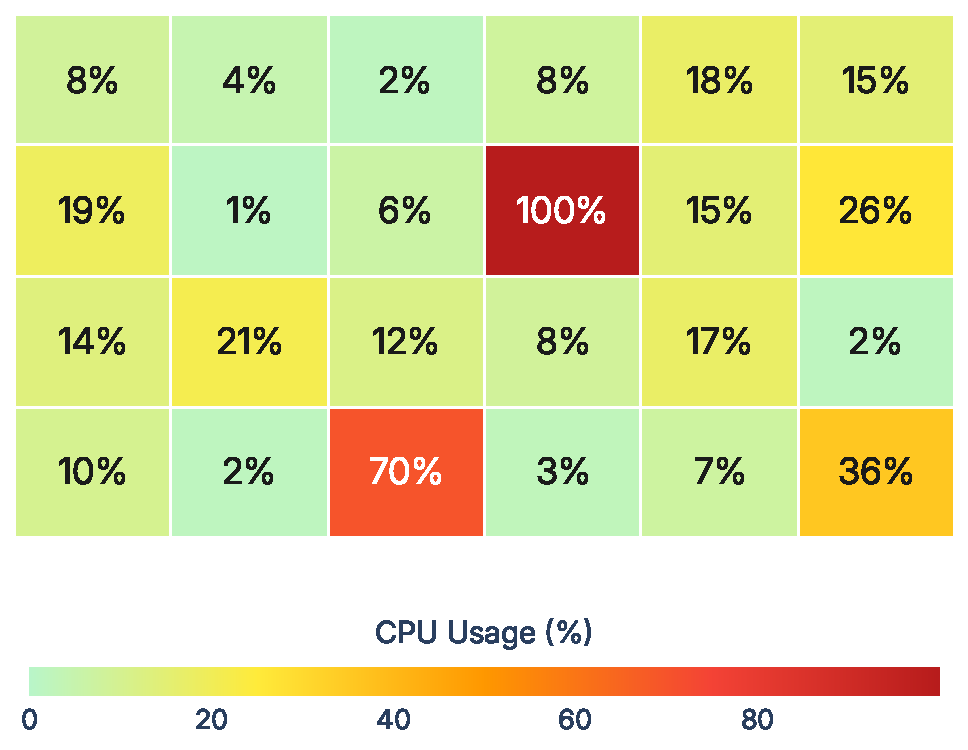
\includegraphics[width=0.5\linewidth]{assets/network/omni_path_cpu_heatmap.pdf}
    \caption[Omni-Path CPU Usage Heatmap]{Heatmap showing all cores with non-zero utilization during performance testing of Omni-Path. The heatmap demonstrates that a single core is fully loaded, while most other cores remain idle or lightly loaded.}
    \label{fig:opa-irq}
\end{figure}

The Omni-Path tuning guide also provides a method for determining the mapping of cores to interrupts~\cite{omni-path-tuning-guide}. Using this, we are able to determine which interrupt types place the most load on the \ac{CPU}. The interrupt mapping is shown in~\cref{fig:omni-path-irq-layout}.

\begin{figure}[H]
    \centering
    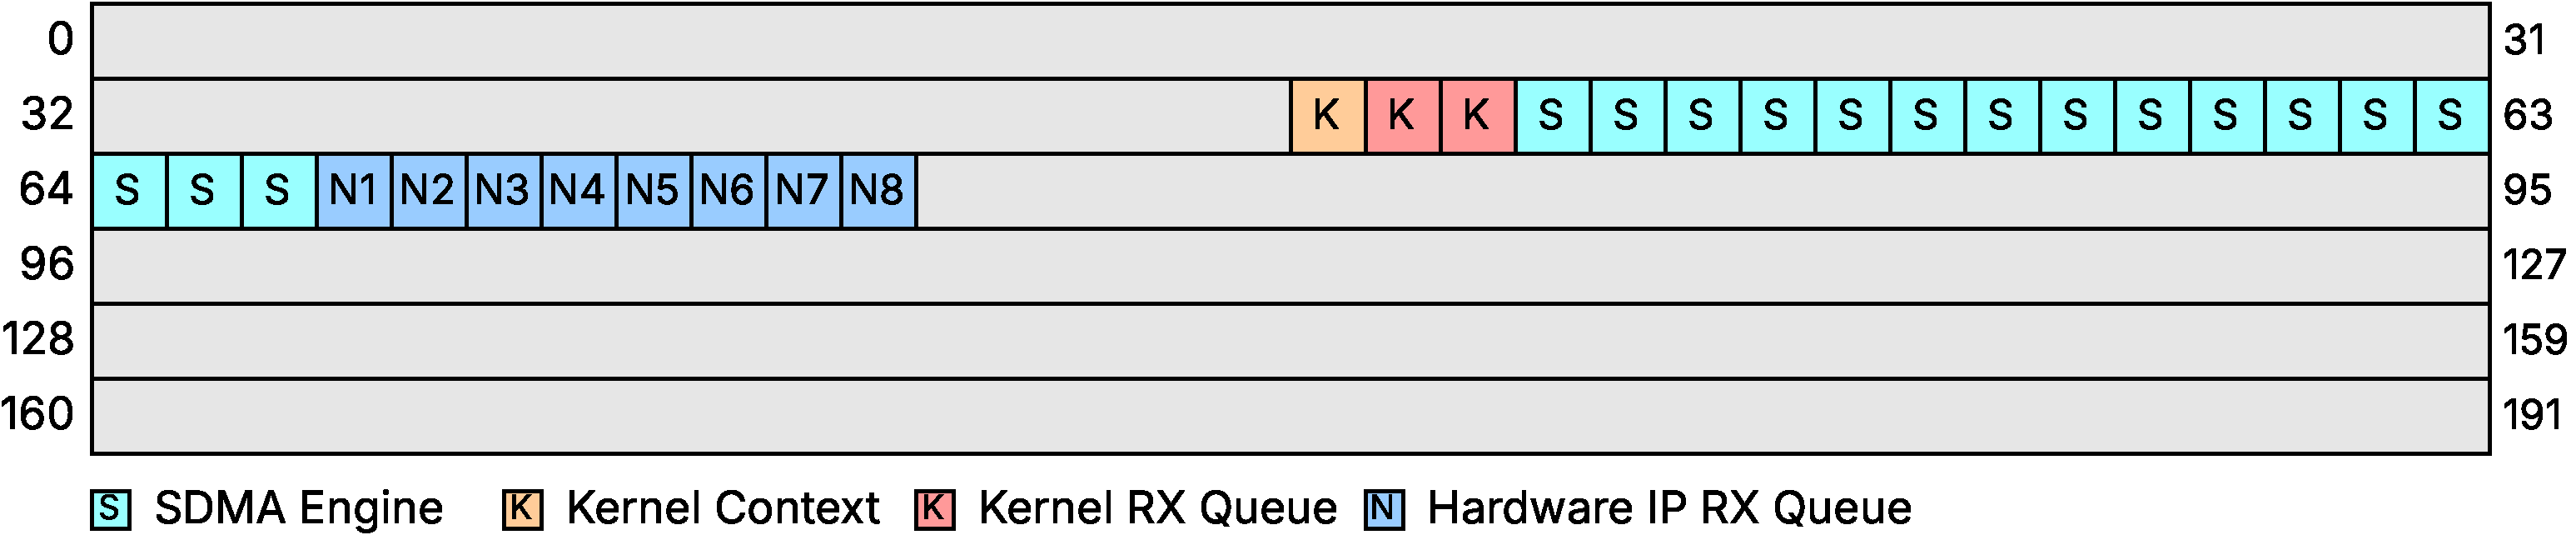
\includegraphics[width=\linewidth]{assets/network/rps/Interrupt-Layout.pdf}
    \caption{Omni-Path IRQ Layout}
    \label{fig:omni-path-irq-layout}
\end{figure}

Based on the interrupt mapping, the performance bottleneck likely stems from the \ac{CPU} usage of interrupts generated to service regular \ac{IP} traffic. This demonstrates that the processing overhead of \ac{IP} over Omni-Path is high due to the interrupt processing. More critically, despite the large number of cores---and therefore, theoretically available network processing performance---the single-core performance remains a performance bottleneck.

Beyond Ceph, these performance limitations can be of particular concern for high-bandwidth \ac{IP} traffic producers and consumers. On the \ac{GWDG} \ac{HPC} cluster, there is an additional network architecture constraint of a 4KB \ac{MTU} for interoperability with InfiniBand hardware, which further increases packet count compared to the maximum supported Omni-Path \ac{MTU} of 10KB. Furthermore, the \acp{CPU} used in the \ac{HPC} cluster are high-core-count \acp{CPU}, which generally have reduced single-core performance compared to, e.g., low-core-count consumer-grade \acp{CPU}. For instance, a consumer-grade Intel \ac{CPU} may run at 6 GHz, while a server-grade \ac{CPU} released during the same time frame may run at 4.1 GHz\footnote{Data from Intel ARK: \url{https://www.intel.com/content/www/us/en/ark.html}. Accessed 03.02 2026. Consumer \acs{CPU}: i9-14900K; Server \acs{CPU}: Xeon Gold 6538N.}.

\subsubsection{Enabling \acs{RPS} with Accelerated \acs{IP}}

The Omni-Path optimization guide recommends enabling either \ac{RPS} or
Accelerated \ac{IP} \cite[p.~77]{omni-path-tuning-guide}. However, given the
interrupt load shown in~\cref{sec:interrupt-handling-issues} as well as the
suboptimal performance, an experimental evaluation of \ac{RPS} in combination
with Accelerated \ac{IP} was performed. To that end, a specialized script was
developed to automatically assign available cores to network queues under the
following constraints:

\begin{itemize}
    \item \ac{RPS} flows can be placed on the same \ac{NUMA} node as the original interrupts to minimize latency, or spread across multiple nodes to potentially improve throughput.
    \item The number of \ac{RPS} flows, as well as the cores on which these \ac{RPS} flows are placed, are adjusted such that they do not overlap with existing interrupts.
    \item The hardware thread for each core is taken into consideration during the placement process to prevent overlaps with the same \ac{CPU} core.
\end{itemize}

\ac{RPS}
flow policies both with and without \ac{NUMA} restrictions were used. The
\ac{NUMA}-restricted placement policy has fewer cores available for \ac{RPS}
flows. However, it benefits from higher bandwidth due to its memory and network
adapter locality. The placement is shown in~\cref{fig:rps-single-numa}.

\begin{figure}[H]
    \centering
    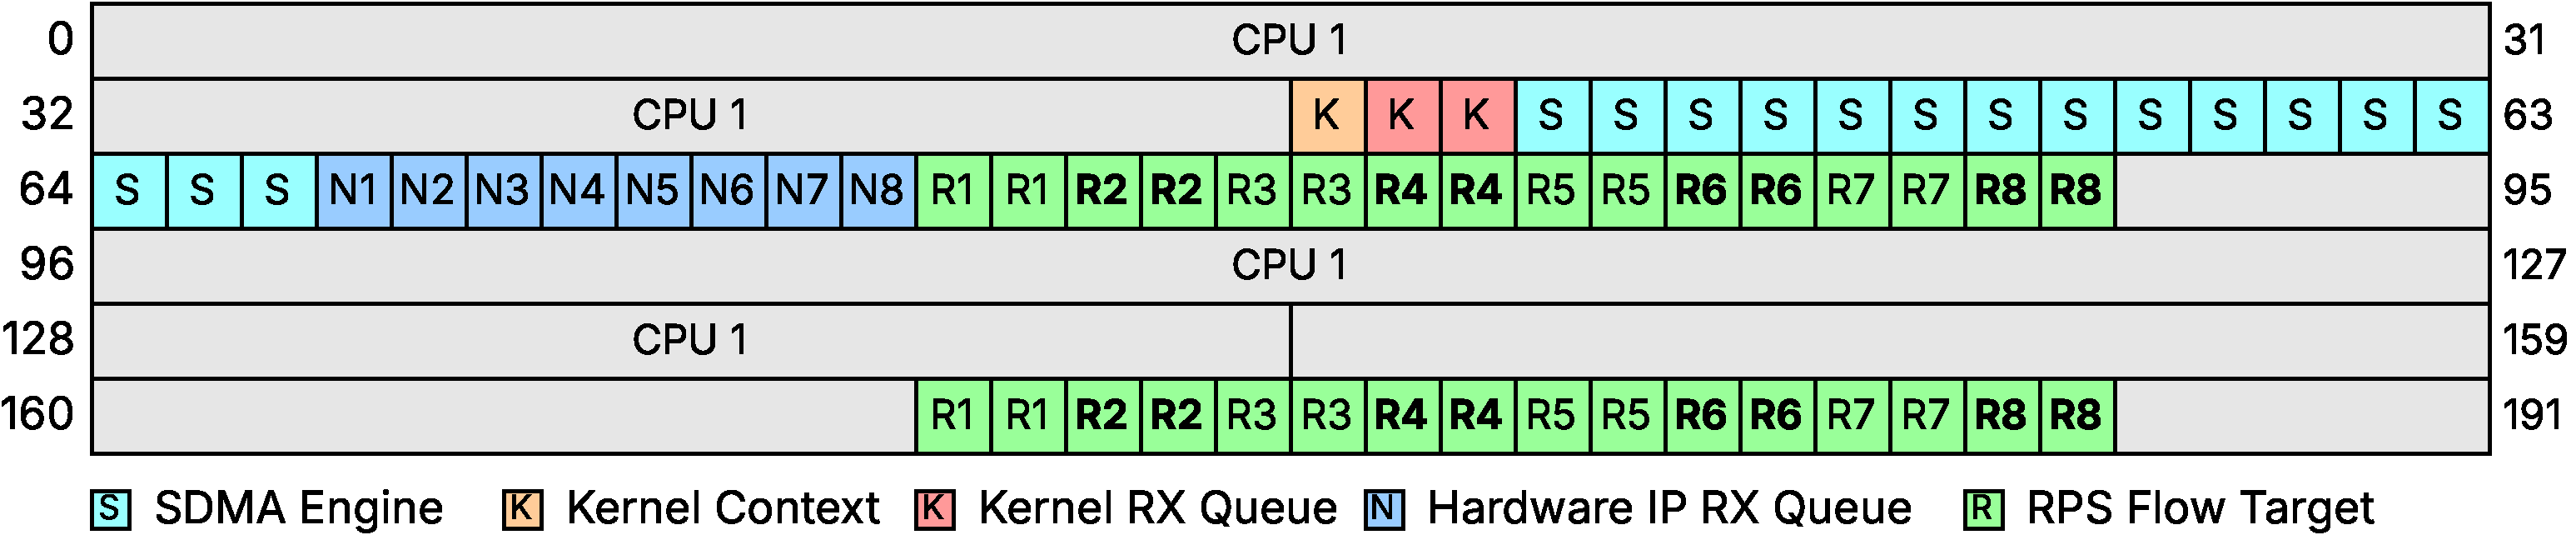
\includegraphics[width=\linewidth]{assets/network/rps/RPS-Single-NUMA.pdf}
    \caption{Single-\acs{NUMA}-Node \acs{RPS} Configuration}
    \label{fig:rps-single-numa}
\end{figure}

The unrestricted \ac{RPS} flow placement is shown in~\cref{fig:rps-multi-numa}.
It has significantly more cores per hardware interrupt to work with, but could
potentially perform worse due to the latency and bandwidth constraints
introduced by the inter-\ac{NUMA}-node link.

\begin{figure}[H]
    \centering
    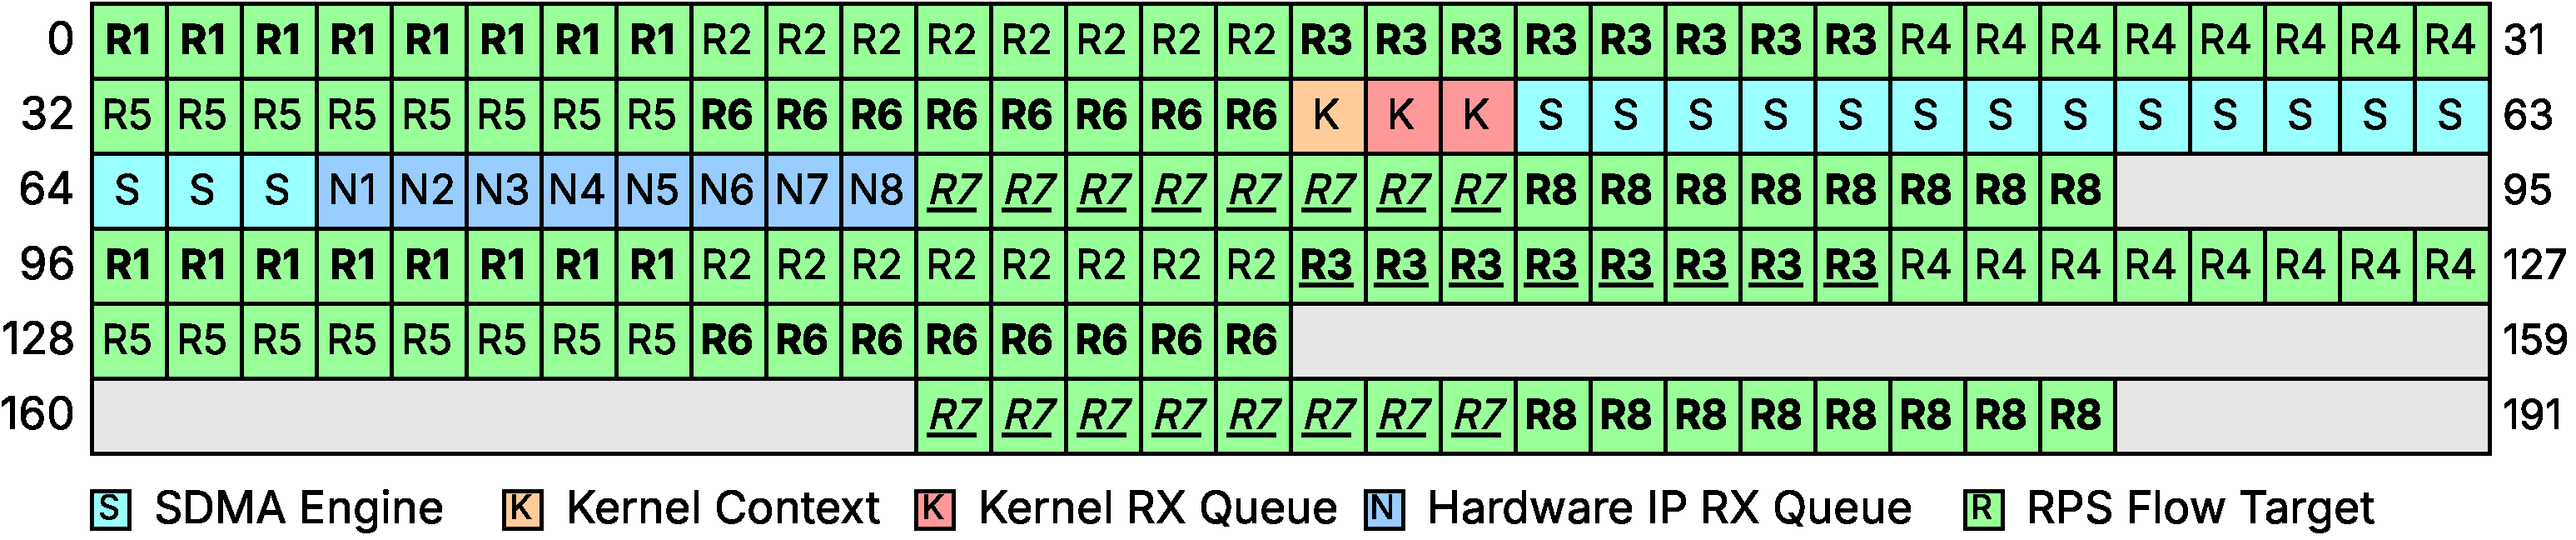
\includegraphics[width=\linewidth]{assets/network/rps/RPS-Multi-NUMA.pdf}
    \caption{Multi-\acs{NUMA}-Node \acs{RPS} Configuration}
    \label{fig:rps-multi-numa}
\end{figure}

% These optimizations were applied to the test nodes and initial testing was
% performed between two Omni-Path equipped test nodes
% (see~\cref{tbl:omnipath-system} for specifications). However, the observed
% performance results were poor.

\subsection{InfiniBand Optimizations}

InfiniBand supports Ceph's \ac{TCP/IP} traffic through its \ac{IPoIB} protocol. While all optimizations as shown in~\cref{tbl:nic-offload} for InfiniBand network adapters were enabled on the tested nodes, the \ac{MTU} was restricted to a maximum of 4000 bytes in order to preserve compatibility with existing infrastructure, such as storage servers and network switches. \Cref{tbl:infiniband-parameters} details the tuned system configuration applied to the test nodes, which were equipped with 200 Gbit/s NVIDIA ConnectX-6 adapters operating in InfiniBand mode.

\begin{table}[h]
\centering
\begin{tabular}{ll}
\hline
\textbf{Parameter}                      & \textbf{Value} \\
\hline
\ac{MTU}                                & 4000 \\
\ac{RPS}                                & Disabled \\
\texttt{irqbalance}                     & Enabled \\
\ac{THP}                                & Always \\
\ac{CPU} Scaling Governor               & Performance \\
\hline
\textbf{Kernel Parameter}               & \textbf{Value} \\
\hline
\texttt{iommu}                          & \texttt{pt} (Passthrough) \\
\texttt{ib\_ipoib.recv\_queue\_size}    & 8192 \\
\texttt{ib\_ipoib.send\_queue\_size}    & 8192 \\
\hline
\textbf{Sysctl Parameter}               & \textbf{Value} \\
\hline
\texttt{net.ipv4.tcp\_rmem}             & 16384 131072 16777216 \\
\texttt{net.ipv4.tcp\_wmem}             & 16384 16384 16777216 \\
\texttt{net.ipv4.rmem\_max}             & 16777216 \\
\texttt{net.ipv4.wmem\_max}             & 16777216 \\
\texttt{net.core.somaxconn}             & 2048 \\
\texttt{net.ipv4.tcp\_mtu\_probing}     & 1 \\
\texttt{net.core.netdev\_max\_backlog}  & 250000 \\


\hline
\end{tabular}
\caption{Configured Parameters for InfiniBand}
\label{tbl:infiniband-parameters}
\end{table}

Manual tuning of software interrupt handling, i.e., \ac{RPS}, was not considered necessary. In contrast to Omni-Path's capabilities, the InfiniBand network adapters supported hardware receive hashing/flow steering with 64 dedicated queues each for send and receive operations, compared to the 8 supported by Omni-Path.
